%%%%%%%%%%%%%%%%%%%%%%%%%%%%%%%%%%%%%%%%%%%%%%%%%%%%%%%%%%%%%%%%%%%%%%%%%%%%%%%
% Capítulo 3: Procedimiento experimental 
%%%%%%%%%%%%%%%%%%%%%%%%%%%%%%%%%%%%%%%%%%%%%%%%%%%%%%%%%%%%%%%%%%%%%%%%%%%%%%%

%Este capítulo ha de contar con seccciones para la descripción de los experimentos 
%y del material.

%También debe haber una sección para los resultados obtenidos y una última de 
%análisis de los resultados.

%++++++++++++++++++++++++++++++++++++++++++++++++++++++++++++++++++++++++++++++
\section{Descripción de los experimentos}
\label{3:sec:1}
\parindent=0.5cm
\raggedright
\subsection{Primer experimento}
El experimento llevado a cabo es la realización de la integral definida, la aproximación
mediante la regla del trapecio y la regla del trapecio compuesta. Compararemos los resultados para ver si se obtiene una aproximacón fiable.
 Veamos\\
Integral definida 
\[
\int_{-1}^{1} \frac{1}{sqrt(2\pi)} \quad\text{e}^{\frac{-x^2}{2}}dx
\]
Regla del Trapecio
\[
\int_{-1}^{} \frac{1}{sqrt(2\pi)} \quad\text{e}^{\frac{-x^2}{2}}dx\approx\left(1-(-1)\right)\frac{f(-1)+f(1)}{2}
\]
Regla del Trapecio compuesta con n=4
\[
h=\frac{1-(-1)}{4} =\frac{1}{2} 
\]
\[
\int_{-1}^{1} \frac{1}{sqrt(2\pi)} \quad\text{e}^{\frac{-x^2}{2}}dx\approx\left[f(-1) + f(\frac-{1}{2}) + f(0) + f(\frac{1}{2} + f(1)\right]
\]


\subsection{Segundo experimento}
En este experimento vamos a ver los distintos errores que puede tomar el teorema para los posibles resultados de $\epsilon$.
Recordamos que $\epsilon$ pertenecerá al intervalo [a,b], en este caso, el intervalo [-1,1].
Por tanto,

\[
-\frac{\left(b-a\right)^3}{12}  \displaystyle f^{(2)}(\epsilon)
\]

para todo $\epsilon$ perteneciente al intervalo [-1,1].



%++++++++++++++++++++++++++++++++++++++++++++++++++++++++++++++++++++++++++++++
\section{Descripción del material}
\label{3:sec:2}
\parindent=0.2cm
\raggedright
El material que hemos empleado para la realización de este proyecto es el lenguaje de
programación Python, para la creación de los programas que verifican este método de integración, 
y el sistema de composición de textos \LaTeX para el diseño del proyecto.


%++++++++++++++++++++++++++++++++++++++++++++++++++++++++++++++++++++++++++++++
\section{Resultados obtenidos}
\label{3:sec:3}
\parindent=0.2cm
\raggedright
\subsection{Resultados del primer experimento}
Los resultados obtenidos son:
Integral definida 
\[
\int_{-1}^{1} \frac{1}{\sqrt(2\pi)} \quad\text{e}^{\frac{-x^2}{2}}dx\approx0.682689 
\]
Regla del Trapecio
\[
\int_{-1}^{1} \frac{1}{\sqrt(2\pi)} \quad\text{e}^{\frac{-x^2}{2}}dx\approx\left(1-(-1)\right)\frac{f(-1)+f(1)}{2}=0.483941
\]
Regla del Trapecio compuesta con n=4
\[
\int_{-1}^{1} \frac{1}{\sqrt(2\pi)} \quad\text{e}^{\frac{-x^2}{2}}dx\approx\left[f(-1) + f(\frac-{1}{2}) + f(0) + f(\frac{1}{2} + f(1)\right]\approx0.882385
\]
\subsection{resultados del segundo experimento}
Tomando varios valores de $\epsilon$,obtenemos la siguinte gráfica:








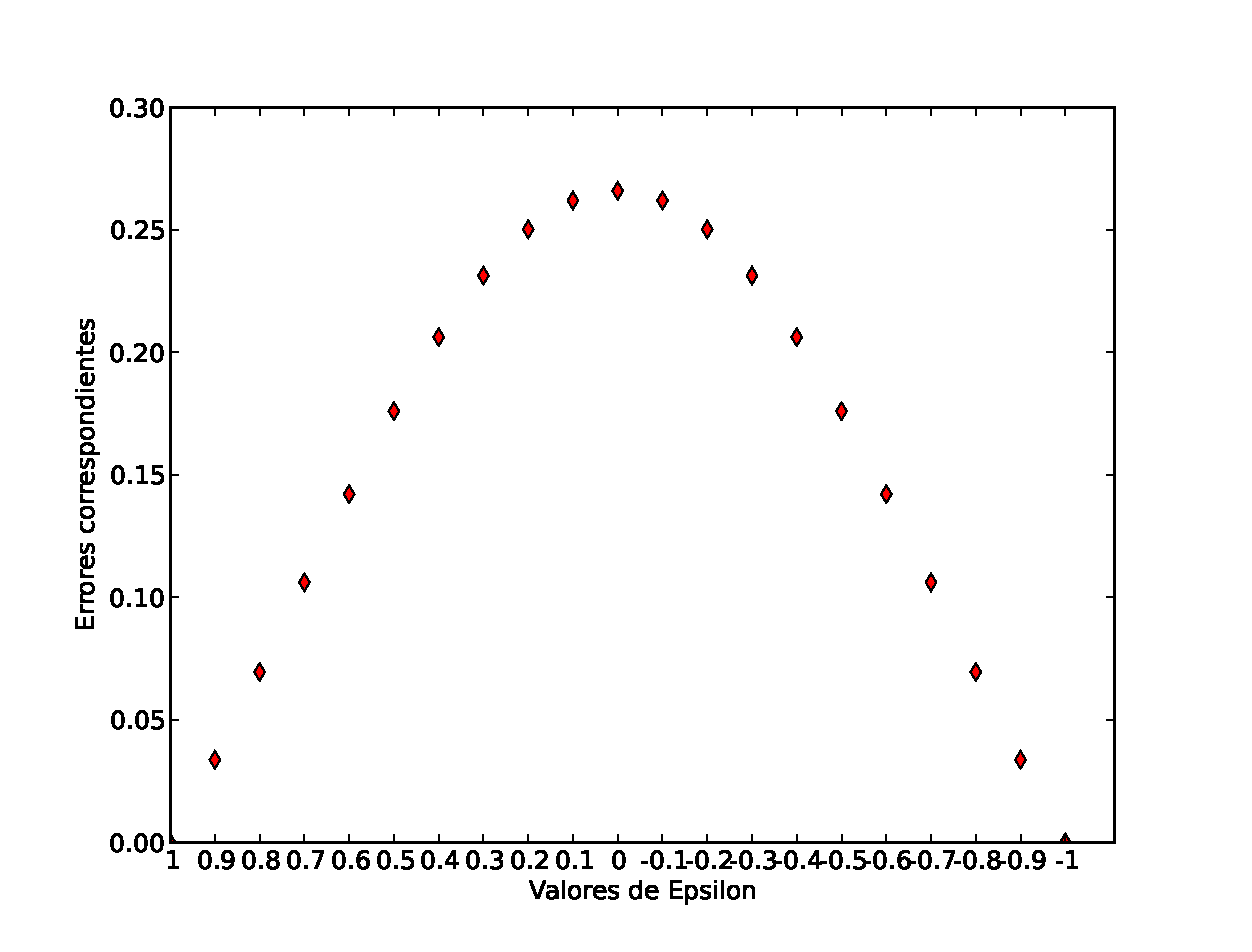
\includegraphics[width=1.25\textwidth]{images/imgraf}
%------------------------------------------------------------
%\begin{figure}[!th]
%\begin{center}
%\includegraphics[width=0.75\textwidth]{images/figura1.eps}
%\caption{Ejemplo de figura}
%\label{fig:1}
%\end{center}
%\end{figure}
%------------------------------------------------------------------------------
Resultados obtenidos en tiempo y velocidad para la regla del trapecio simple y la regla del trapecio compuesta
%--------------------------------------------------------------------------
\begin{table}[!ht]
\begin{center}
\begin{tabular}{|c|c|} \hline 
\textbf{Tiempo por Trapecio simple} & \textbf{Tiempo por trapecio compuesto} \\ 
\textbf{(en s)} & \textbf{(en s)} \\ \hline \hline
0.1412169 &
0.1414737
\\
\hline

0.1414649 &
0.1415798
\\
\hline

0.1412210 &
0.1413900
\\
\hline


\end{tabular}
\end{center}
\caption{Resultados experimentales de tiempo (s) y velocidad (m/s)}
\label{tab:1}
\end{table}


%------------------------------------------------------------------------------

%++++++++++++++++++++++++++++++++++++++++++++++++++++++++++++++++++++++++++++++
\section{Análisis de los resultados}
\label{3:sec:4}
\parindent=1cm
\raggedright
 
